\chapter{Neural Machine Translation: a review}
\label{chap:nmt-review}
In this chapter, we briefly review some basic knowledge of Neural Machine Translation (NMT) which provides the foundation for the experiments of this thesis. Neural Machine Translation was first introduced in 2014 via the work of \citet{Cho14properties,Bahdanau15learning}. Since then, NMT has been largely developed and outperformed old approaches, including Rule-based Machine Translation (RBMT\nomenclature[rbmt]{RBMT}{Rule-based Machine Translation}) and Statistical Machine Translation (SMT) in high-resource languages such as French-English or English-German.

Building a Neural Machine Translation model consists of 3 basic steps, including text tokenization (Section \ref{sec:tokenization}), training NMT model with pairs of tokenized source and target sentences (Section \ref{sec:train}) and decoding or translating (Section \ref{sec:inference}). In the first step, each sentence is transformed into a sequence of tokens, which can be words, sub-words, or characters (Section \ref{sec:preprocessing}). The sequence of tokens will be transformed into a sequence of integers. In the second step, given a choice of neural architecture (Sections \ref{sec:rrn}, \ref{sec:cnn} or \ref{sec:transformer}); the parameters of the NMT model are optimized according to a training objective (Section \ref{sec:train}). The input of the NMT model during the training consists of a pair of sequences of integers corresponding to a pair of source and target sentences. In the final step, when the NMT model is learned, given any sentence in the source language, the NMT model generates a translation via a decoding algorithm (Section \ref{sec:inference}) such as beam search \citep{Koehn04pharaoh}. In the inference step, the input of the NMT model is only the sequence of integers corresponding to the source sentence.

\section{Text preprocessing for NMT \label{sec:tokenization}} \label{sec:preprocessing}
Text preprocessing includes two steps, including text normalization and text tokenization. Text normalization aims to transform a text into a single canonical form. Text tokenization transforms a sentence into the input format of the NMT model. In practice, text normalization is optional, while text tokenization is obligatory.

The tokenization process consists of transforming a sentence into sequence of symbols called tokens, which will be transformed into sequences of integers and then be served as the input of the NMT model. Text tokenization is an essential step in NMT and needs to be carefully conducted. We have to tokenize sentences because NMT models only take a sequence of integers as input. In practice, a token can be a word or a part of a word. There are three common types of token: words, sub-words, and characters. These tokens are indexed by a predetermined vocabulary so we can map each token to an integer. The sequence of tokens is converted into a sequence of integers $IDs \in V$ where V is the set of indices of the corresponding vocabulary. The vocabulary of the NMT model is fixed. Any out of vocabulary (OOV \nomenclature[oov]{OOV}{Out of vocabulary}) token is mapped to a special token $<UNK>$, which stands for unknown. The size of the vocabulary of an NMT model is chosen to balance the coverage over the processed tokens with a practical constraint on the size of the model. The vocabulary of an NMT model is usually limited to 30-40 thousand types. In the following discussion, we denote $\Sigma_{x}$, $\Sigma_y$ the source vocabulary and the target vocabulary, respectively. \nomenclature[$\Sigma_{x}$]{$\Sigma_{x}$}{source vocabulary} \nomenclature[$\Sigma_{y}$]{$\Sigma_{y}$}{tgt vocabulary}. The tokenization process needs to be reversible. To get the final translation, we convert the sequence of tokens predicted by the NMT model into a normal sentence.
\subsection{Word tokenization}
Word tokenization identifies all unique words in the respective training sets to construct the source and target language vocabularies. Because of the computational constraints, the vocabulary of an NMT model is typically limited to a few tens of thousands of types. The types found in the training sets will be reordered according to their frequency, and the top $V$ most frequent types are selected to form a vocabulary \citet{Cho14properties}. This tokenization algorithm has the disadvantage that its coverage is relatively small. Consequently, word-based NMT models usually have to scope to out-of-vocabulary tokens \citet{jean15using,luong15addressing,Li16towards}.

\subsection{Subword tokenization}
Subword tokenization is the process of finding an optimal segmentation of words such that a limited set of word-pieces can segment a large vocabulary. The rationale behind the sub-word tokenization is that words are usually composed of several morphemes. For example a plural countable noun is composed of its root and the affix "s". By separating the root and the affix, we avoid adding both the singular and the plural form of a noun in our vocabulary and reduce the size of it. In practice, subword tokenization largely increases the coverage of the vocabulary and efficiently handles unseen words. The vocabulary can be built by applying the morphological rules of the language or can be learned by heuristic algorithms such
as Byte pair encoding (BPE \nomenclature[bpe]{BPE}{Byte Pair Encoding})\citep{Gage94anew,Mike12japanese,Sennrich16neural}. The two more popular sub-word tokenizations are the BPE tokenization \citep{Gage94anew, Mike12japanese,Sennrich16neural} and Sentence-piece tokenization \citep{Taku18subword}, which are based on 2 different approaches: frequency-based and sampling-based respectively.

BPE tokenization is based on the following algorithm. Given a corpus and an upper bound $K$ of the number of merge operations, BPE tokenization learns a set of at most $K$ merge operations and a set of subwords that allows the formation of any word in that corpus. In principle, words are first segmented into sequences of characters. At each iteration, the BPE algorithm counts the occurrences of each pair of the current types (characters in the beginning), then adds the merge operation of the most frequent pair to its operation set. Next, it redefines the segmentation of every word according to the new operation set and moves to the next iteration. The algorithm stops when it reaches the upper bound $K$. In the end, frequent words remain unsegmented while rare words become sequences of BPE types. Given a set of BPE operations, BPE tokenization segments a word by first segmenting it into a sequence of characters and then applying merge operations to the characters. BPE operations can be learned jointly from both the source and the target languages, from multiple languages as in multi-lingual NMT or separately from each language. Despite the efficacy in the open-vocabulary NMT, BPE tokenization has one default as it allows one word having different BPE encodings \citep{Taku18subword} which the NMT model handles as entirely different inputs.

Sentence-piece tokenization also allows many different segmentation candidates for one word but uses a unigram language model to assign a probability to each word segmentation candidate. The motivation of sentence-piece is to enable the NMT model to be trained with multiple segmentation candidates, which will be sampled from a learned distribution over possible candidates. Applying sentence-piece tokenization on the fly allows the NMT model to be robust against the ambiguity raised from the existence of multiple sub-word encoding candidates of a word. 

Besides sentence-piece and BPE, there are alternative paradigms for sub-word tokenization such as syllabification \citep{Assylbekov17syllable} or linguistically informed tokenization \citep{Ataman17linguistically, Huck17target, Machcek18morphological}.
\subsection{Character tokenization}
Character tokenization segments words into sequences of characters. This tokenization circumvents the problem of finding an optimal sub-word segmentation for multiple languages in multilingual NMT. Furthermore, character tokenization reduces the size of the vocabulary to a small number of written characters. However, the length of the resulting sequence increases significantly as words are extremely split into character units. As a result computational requirements during training and decoding time increase. First studies on the character-based NMT , including the work of \citet{Wang15character,Luong16achieving}, focused on solving the out-of-vocabulary and softmax bottleneck problems associated with word-level models. \citet{Costa16character, Chung16character, Lee17fully, costa17byte} proposed variants of character-based model.
\subsection{Byte-level tokenization}
Byte-level tokenization is used to segment the byte-level representation of the text. The rationale behind this tokenization is that byte-level representation could handle character-rich languages such as Japanese and Chinese. However, for the same sentence, the byte-level representation is usually much longer than the character-level representation. Furthermore, taking a sequence of bytes as the input of the NMT model greatly increases the cost. To reduce the length of the input sequence, byte-level tokenization applies BPE tokenization on sequences of bytes. In practice, \citet{Wang19neural} showed comparable performance of byte-level BPE-based NMT compared to BPE-based NMT. 
\section{NMT's main components}
\nomenclature[lm]{LM}{Language modeling or Language model}
In principle, an NMT model consists of 3 parts: 1) a look-up table of word embeddings, 2) an encoder and 3) a decoder. Similar to the SMT approach, an NMT model modelizes the conditional probability of the target sequence given the source sequence, i.e. $P(y|x)$ in which $x=[x_0,\cdots,x_{I}], y=[y_0,\cdots,y_{J}]$. Most existing NMT models are auto-regressive, i.e., $P(y|x)$ is factored into a product of a chain of conditional probabilities which predict a target token given the previous predicted target tokens and the source sequence as
\begin{equation}
P(y|x) = \displaystyle{\mathop{\prod}_{i=1}^{J}} P(y_i|y_{<i},x).
\label{eq:factorization-chap2}
\end{equation}
We always assume that the target sentence is initialized by a special token named "begin-of-sentence" $<BOS>$, hence, $y_{0}=<BOS>$. \nomenclature[bos]{BOS}{begin-of-sentence}

The encoder maps the source sequence $x$ to an intermediate representation in a continuous high dimensional vector space. The Decoder takes the representation of the source sequence $Enc(x)$ as input to condition its prediction on the source sequence. At each time step $i$, the decoder outputs a distribution over the target vocabulary by mapping its $i^{th}$ hidden state to vector space $\mathbb{R}^{|\Sigma_y|}$ where $\Sigma_y$ is the target vocabulary
\begin{equation}
\begin{array}{rcl}
P(.|y_{<i},x) = \operatorname{softmax}(Linear(s_i)),
\end{array}
\end{equation}
where $Linear$ is a dense layer mapping to $\mathbb{R}^{|\Sigma_y|}$.

The hidden state of the Decoder is computed recursively as 
\begin{equation}
s_i = g(s_{i-1},y_{i-1},c_i),
\end{equation}
using the hidden state of the previous time step, the observation of the previous time step (i.e. the $(i-1)^{th}$ token) and the context $c_i$, which is computed from the representation of the source sequence $Enc(x)$ and $s_{i-1}$.

In order to transform the input sequence of integers into continuous hidden states, Encoder and Decoder have to use a look-up table of word embeddings. A word embedding is a real-valued vector in a high dimension space that represents a token in the vocabulary of the NMT model. The motivation of using word embedding is to transform the input sequence of integers to a sequence of vectors in a continuous space which allows the parameters of the NMT model to be trained with gradient descent-based optimization methods. The lookup table has the size of $|\Sigma_{\{x,y\}}| \times d$ where $|\Sigma_{\{x,y\}}|$ is the size of the corresponding vocabulary, and d is the dimension of word embedding space. Word embeddings are not only used in NMT models but also in Neural language models \citep{Bengio03aneural}(NLM\nomenclature[nlm]{NLM}{Neural Language Model}). \citet{Le12continuous, Schwenk12continuous} used NLM for phrase-based statistical machine translation. Moreover, word embedding can be trained alone using the Skip-gram model \citep{Mikolov13distributed} or the Continuous Bag of Word model \citep{Mikolov13efficient}. After training such models, the resulting word embeddings possess semantic properties so that words having similar meanings or close meanings are mapped to similar vectors in terms of cosine similarity \citep{Collobert11natural, Mikolov13distributed, collobert08aunified}. The fine-grained semantic representation of word embeddings significantly improves the performance of AI in text classification, text retrieval, etc., and surprisingly enables unsupervised machine translation and unsupervised word translation  \citep{Pennington14glove,levy15improving,Guillaume18unsupervised,santos20word}. By using word embeddings, the source sequence is mapped to a sequence of real-valued vectors. 

The encoder encodes the source sequence of word embeddings to another sequence of real value vectors (hidden states or contextualized embeddings) \citep{Cho14properties,Bahdanau15learning,Vaswani17attention}, in a high dimension space called a latent space. This process aims to mix the representation of each token with ones of the context surrounding that token. The context of a word is the set of words surrounding that word. Combining the representation of a word with its context allows the NMT model to condition the translation of that word on its context. The encoder can combine the state of the token with one of its preceding tokens in a Recurrent encoder, with ones of the surrounding window in a Convolutional encoder, or with ones of the whole sentence in an Attention-based encoder. We illustrate the range of context captured by those three encoders in figure \ref{fig:encoding}. Each encoding paradigm has its advantages and disadvantages. The Recurrent encoder respects the order of tokens because it consumes tokens one by one from left to right. However, it is very slow to encode the input sequence. Convolutional encoder and Attention-based encoder encode all input tokens simultaneously that brings a great advantage in speed. But allowing direct connections between states prevents Convolutional encoders and Attention-based encoders from apprehending the sequence's order. Therefore they have to use positional embedding to know the position of each token. 

\begin{figure*}[htbp]
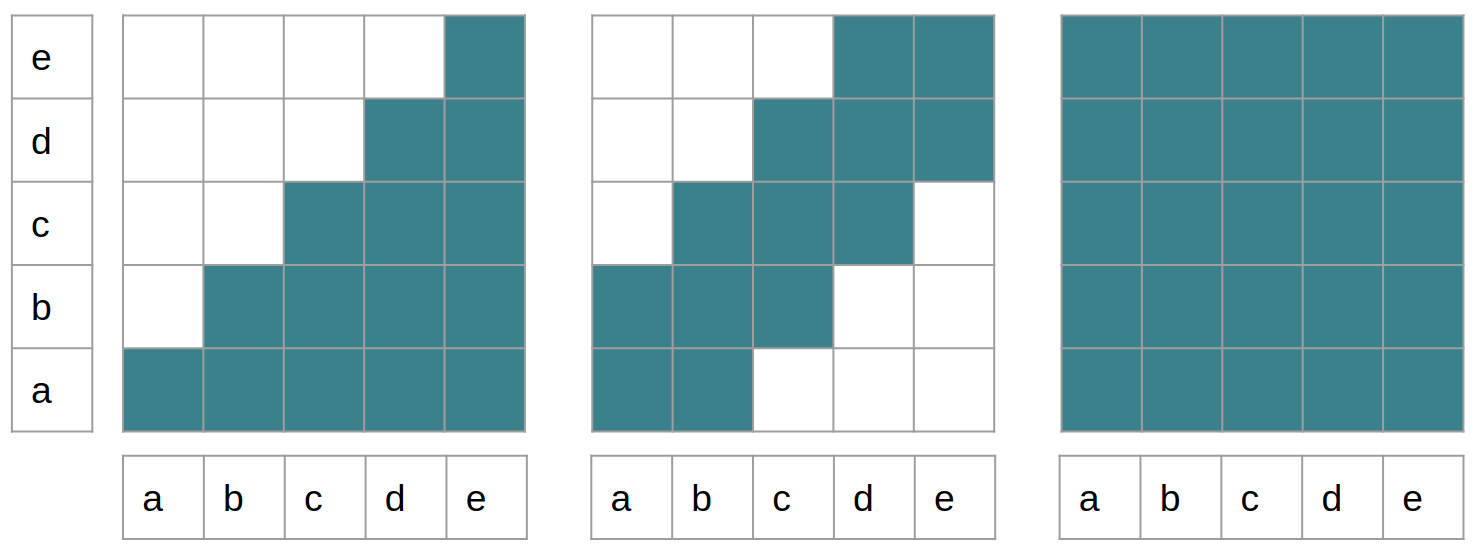
\includegraphics[width=\textwidth]{graphics/encoding.png}
\caption[Illustration of context range at each token in different encoding mechanism]{Illustration of context range at each token in different encoding mechanism. From left to right: Recurrent encoder, Convolutional encoder, Attention-based encoder. The example sequence is $[a,b,c,d,e]$ and each colored column represent the context range of the corresponding token.}
\label{fig:encoding}
\end{figure*}

The decoder works similarly to a language model as it predicts one token per time step. However, the decoder conditions its prediction on the source sequence. Therefore, the decoder takes the output of the encoder as its inputs. An Auto-regressive decoder conditions its prediction on the predictions of previous steps and the source sequence. Because all of our experiments use auto-regressive NMT, from now, a decoder is an auto-regressive decoder if there is no other specification. The decoder usually uses the same neural architecture as the encoder. However, unlike the encoder, the range of context of a token is strictly limited to its preceding tokens. Because the hidden state of the decoder is computed from the previous hidden states and the observation of the previous step, we need to initialize the $0^{th}$ hidden state $s_0$ (optional) and the $0^{th}$ token. That is why we always begin the target sequence by the token $<BOS>$, and the decoder starts predicting from the second token on. For example, if $[a,b,c,d,e]$ is predicted by the decoder, the prediction of token $a$ is conditioned by source sequence $x$ and $<BOS>$; the prediction of token $b$ is conditioned by source sequence $x$ and $[<BOS>,a]$ and so on. Besides, the decoder needs a signal to stop its generative prediction. We always end a prediction by "end-of-sentence" token or $<EOS>$. Therefore, instead of predicting $[a,b,c,d,e]$, the decoder predicts $[a,b,c,d,e, <EOS>]$. Concerning the construction of hidden states, the Recurrent decoder usually initializes $s_0$ by the last hidden state of the encoder followed by a linear transformation. In contrast, the Convolutional decoder and the Attention-based decoder do not need to initialize $s_0$ as every hidden state directly accesses the predictions preceding its time step without going through its preceding state. We illustrate the difference between decoding paradigms in the figure \ref{fig:decoding}.

\begin{figure*}[htbp]
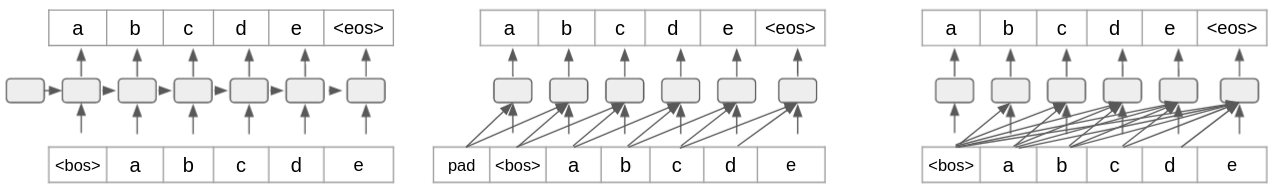
\includegraphics[width=\textwidth]{graphics/decoding.png}
\caption[Illustration of 3 most popular auto-regressive decoding paradigms]{From left to right: Recurrent decoder, Convolutional decoder, Attention-based decoder. The example sequence is $[a,b,c,d,e]$. The figure illustrates only one layer of the decoder.}
\label{fig:decoding}
\end{figure*}

NMT's architectures are usually a stack of multiple layers. As described above, the input source sequence is mapped to a sequence of word embeddings. This is considered the $0^{th}$ layer of the Encoder. The $i^{th}$ layer is built upon the $(i-1)^{th}$ layer by applying the same encoding mechanism, which can be recurrent layer, convolutional layer or self-attention layer, to the output of the $(i-1)^{th}$. We illustrate different multi-layer decoders in figure \ref{fig:multi-layer}. For example, \citet{Vaswani17attention} stacked 6 Transformer layers in both the encoder and the decoder of their NMT model. Deep NMT models are able to learn from very large-scale of parallel data \citep{Ott18scaling} and continually create new state-of-the-art performances. However, deep NMT models are harder to train because the gradient flow has to back-propagate through many layers. In order to prevent the gradient flow from vanishing, which happens when the value of the output of the linear transformation in some layer jumps outside the domain of the activation function, \citep{He16deep} proposes using residual connections, which replaces $f(x)$ by $f(x)+x$ where $x$ is the output of the lower layer and $f(.)$ is the transformation of the layer, to transit from the lower layers to their following layers. By using residual connections, a fraction of the gradient still reaches the lower layer and continues to propagate until the lowest layer.

Deep NMT models also suffer from Internal Covariate Shift in which the distribution of the value of each layer significantly changes due to the change of the parameters of the models. In deep neural network, the distribution of the value of high layers is highly affected by the parameters of the lower layers and can be dramatically shifted by a small change in the value of those parameters. Large shift can push the value of the layer to the saturation zone of activation function where the gradient is extremely small. In practice, the saturation problem can be mitigated by using the Rectified Linear Units $RELU(x) = max(x,0)$ \citep{Nair10rectified}. Recently, \citep{Ioffe15batch,Jimmy16layer} propose different normalization methods to stabilize the value of layers so that they are not easily pushed to saturation zone of activation function. In principle, Normalization methods re-scale and re-center the distribution of the value of each layer with learnable mean and learnable variance. Normalization methods prove to be very helpful in practice. For example, Layer normalization must be included in every layer of Attention-based NMT \citep{Vaswani17attention}.

\begin{figure*}[htbp]
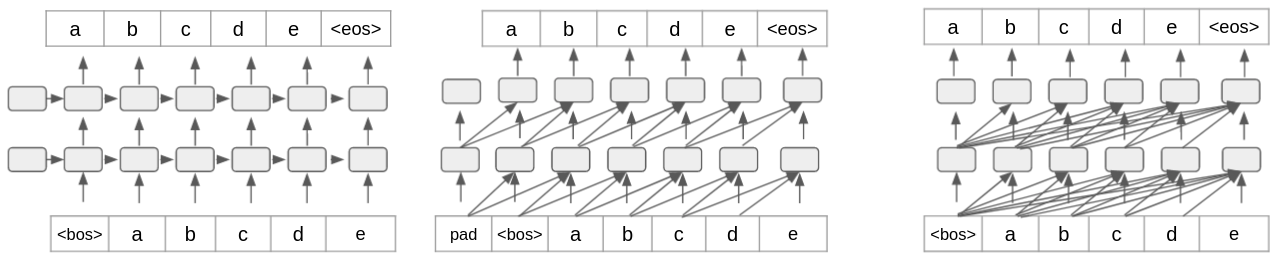
\includegraphics[width=\textwidth]{graphics/multi_layer_decoder.png}
\caption[Illustration of 3 most popular multi-layer auto-regressive decoding paradigms]{From left to right: Recurrent decoder, Convolutional decoder, Attention-based decoder. The example sequence is $[a,b,c,d,e]$. The figure illustrates only two layers of the decoder.}
\label{fig:multi-layer}
\end{figure*}

\section{Recurrent neural machine translation} \label{sec:rrn}
\nomenclature[rnn]{RNN}{Recurrent neural network}
This section reviews the very first NMT architecture, the Recurrent neural machine translation architecture (RNMT\nomenclature[rnmt]{RNMT}{Recurrent neural machine translation}). RNMT is composed of a Recurrent encoder, a Recurrent decoder, and tables of word embeddings. The Recurrent encoder and the Recurrent decoder usually use the same type of Recurrent neural network (RNN) layers, such as Gated recurrent unit (GRU) and Long-short term memory (LSTM), which we will explain in the following section. RNMT is strictly auto-regressive as each hidden state in the encoder/decoder has to go through every intermediate state to assess the information of any time step before it. The hidden states of RNMT inherit the ordering information, which is an advantage over Convolutional neural machine translation (CNMT\nomenclature[cnmt]{CNMT}{Convolutional neural machine translation}) and Attention-based neural machine translation (ANMT\nomenclature[anmt]{ANMT}{Attention-based neural machine translation}). However, a lack of straightforward connections between the positions of the input sequence causes many difficulties in the training of RNMT, for example the vanishing gradient problem in backpropagation through time \citet{Pascanu13onthe}.

\subsection{GRU, LSTM layers}
\nomenclature[gru]{GRU}{Gated recurrent unit}
\nomenclature[lstm]{LSTM}{Long-short term memory}
Gated recurrent units (GRU) and Long-short term memory units (LSTM) are the two most popular layers in the group of Recurrent neural networks. They follow the auto-regressive paradigm by constructing the hidden states one by one as follows
\begin{equation}
\begin{array}{rcl}
h^l_t = f(h^{l-1}_t, h^l_{t-1})
\end{array}
\end{equation}
where $h^{l-1}_t$ is the hidden state at time step $t$ of the $(l-1)^{th}$ layer, the $0^{th}$ layer is the sequence of word embeddings; the mapping $f$ can be GRU cell or LSTM cell, which will be explained below.

LSTMs were first introduced by \citet{Hochreiter97long}. They use 4 gating functions including input gate i, output gate o, forget gate $f$ and memory cell $c$. At each time step $t$, the contextualized embedding $h_t$ is computed as follows
\begin{equation}
\label{eq:lstm}
\begin{array}{rcl}
f_t &=& \sigma_g (W_f h^{l-1}_t + U_f h_{t-1} + b_f),\\
i_t &=& \sigma_g (W_i h^{l-1}_t + U_i h_{t-1} + b_i),\\
o_t &=& \sigma_g (W_o h^{l-1}_t + U_o h_{t-1} + b_o),\\
\tilde{c}_t &=& \sigma_c (W_o h^{l-1}_t + U_o h_{t-1} + b_o),\\
c_t &=& f_t \odot c_{t-1} + i_t \odot \tilde{c}_t,\\
h_t &=& o_t \odot \sigma_h(c_t),\\
\end{array}
\end{equation}
where $\sigma_g$ is the sigmoid function, $\sigma_c$ is the hyperbolic tangent function, $\sigma_h$ is either the hyperbolic tangent function or the identity function and $\odot$ is the element-wise multiplication. These functions are applied element-wise to intermediate vectors in the equations.

The motivation behind this highly complex structure is to stabilize the exploding/diminishing gradient flow \citep{Pascanu13onthe} induced by back-propagation through time (BPTT \nomenclature[bptt]{BPTT}{Back-propagation through time}) \citep{Hochreiter97long}. The second architecture GRU, which was proposed by \citet{Cho14properties}, mitigates the complexity of LSTM by using only three gates as follows.
\begin{equation}
\label{eq:gru}
\begin{array}{rcl}
z_t &=& \sigma_g (W_z h^{l-1}_t + U_z h_{t-1} + b_z)\\
r_t &=& \sigma_g (W_r h^{l-1}_t + U_r h_{t-1} + b_r)\\
\hat{h}_t &=& \sigma_h (W_h h^{l-1}_t + U_h (r_t \odot h_{t-1}) + b_h)\\
h_t &=& (1-z_t)\odot h_{t-1} + z_t \odot \hat{h}_t\\
\end{array}
\end{equation}
Where $\sigma_h$ is a hyperbolic tangent function while other notations are the same as in the equations \ref{eq:lstm}.
\subsection{RNN encoders}
RNN encoders use LSTM or GRU layers to encode the source sequence. RNN encoders can use more than one layer to capture more fine-grained language representations \citep{Li20shallow}. The $0^{th}$ layer is a sequence of word embeddings, which are extracted from the look-up table of the source side using the word ordering provided by the source sequence. 

\subsubsection{Bidirectional RNN encoder}
Unlike the decoder, the encoder is not constrained to process the input sequence from left to right. Effectively, the context of one token in the source sequence contains not only its preceding neighbors but also its following neighbors. Therefore, encoding the source sequence from left to right is not enough to fully describe the context of each token. To increase the coverage of contextualized embedding, the encoder process the source sequence both from left to right and from right to left at the same time. Such encoders are deemed bidirectional. Bidirectional encoding results in two sequences of contextualized embeddings; the encoder simply combines two contextualized embeddings of a token into one real vector via either concatenation or summation. The resulting contextualized embedding improves the representation of each word with information regarding its neighbours on the right and on the left.
\subsection{RNN decoders}
RNN decoders predict the target sequence from left to right, one token per time step. It initializes the $0^{th}$ hidden state by zero vector or a linear transformation of the last hidden state of the last layer of the encoder. The following section will discuss on an important component of the NMT model, which are attention mechanisms. As the hidden representation of the decoder at each step is computed as follows
\begin{equation}
s_i = g(s_{i-1},y_{i-1},c_i),
\end{equation}
where $c_i$ is the context vector. $c_i$ is computed via an attentional mechanism using $s_i$ and $Enc(x)$, which will be explained in Section \ref{ssec:attention}.

The prediction probability will be computed as follows
\begin{equation}
p(y_i|s_i,y_{i-1},c_i) = \operatorname{softmax}(Dense(t_i))_{y_i}
\end{equation}
where $y_i$ is an index of the target vocabulary, $Dense$ is a dense layer, whose output is of dimension $|\Sigma_y|$, and $t_i$ is computed as follows
\begin{equation}
\begin{array}{rcl}
t_i &=& \big[ max\big\{ \tilde{t}_{i,2j-1}, \tilde{t}_{i,2j} \big\} \big]^{T}_{j=1,\cdots,d}, \\
\tilde{t}_i &=& U_0 s_{i-1} + V_0Emb(y_{i_1}) + C_0c_i,
\end{array}
\end{equation}
where $Emb(y_{i-1})$ is the word embedding of the token $y_{i-1}$, $U_0 \in \mathbb{R}^{2l\times d}$, $V_0 \in \mathbb{R}^{2l\times d'}$, and $C_0 \in \mathbb{R}^{2l\times d}$ for a uni-directional encoder and $C_0 \in \mathbb{R}^{2l\times 2d}$ for a bi-directional encoder.
\subsubsection{Attention mechanisms \label{ssec:attention}}
An attentional mechanism consists of 3 components: Query vectors, Key vectors, and Value vectors. Given a sequence $Q_i$, $i \in [1 \cdots n]$, $K_j$, $j \in [1 \cdots m]$ and $V_j$, $j \in [1 \cdots m]$, the results
of the attentional mechanism composed by those vectors will be as follows
\begin{equation}
\operatorname{Attention}(Q,V,K)_i = \displaystyle{\mathop{\sum}_{j=1}^{m}} \frac{exp(sim(Q_i,K_j))}{\displaystyle{\mathop{\sum}_{p=1}^{m}}exp(sim(Q_i,K_p))}*V_j, i \in [1, \cdots, m],
\end{equation}
where the function $sim(x,y)$ can be the standard dot product $<x,y>$ \citep{Vaswani17attention}, a generalized dot product $<x,W_a*y>$ or $<v_a, tanh(W_a*[x,y])>$ \citep{Luong15stanford, Bahdanau15learning}.

The attention mechanism manages and quantifies the dependences between the input sequence and the output sequence (e.g., source contextualized embeddings and target contextualized embeddings), or the input sequence itself (e.g., self-attention layers in Transformer \citep{Vaswani17attention}). In the RNN MT model, the attentional mechanism is used to capture the dependences of each token in the target sequence on the tokens in the source sequence. For example, \citet{Bahdanau15learning} computed a context vector at $i^{th}$ time step in the decoder as follows
\begin{equation}
\begin{array}{rcl}
c_i &=& \sum_{j} \alpha_{ij} h_j, \\
\alpha_{ij} &=& \frac{exp(e_{ij})}{\sum_{k}exp(e_{ik})}, \\
e_{ik} &=& sim(s_{i-1},h_k),\\
\end{array}
\end{equation}
where $h_j$ is the output of the last layer of the encoder, $s_{i-1}$ is the hidden state at the $(i-1)^{th}$ time step of the last layer of the decoder. 

%This context vector will be used to compute the hidden state at $i^{th}$ position by the attentional mechanism improves the translation quality of very long sequences. Indeed, the context vector produced by the RNN encoder struggles to capture all the dependence between tokens of the input sequence because it lacks the direct links between 2 tokens. The information of a token vanishes while the encoder moves toward the far ending of the input sequence. The same problem happens with the decoder when it decodes the context vector into the output sequence. The attentional mechanism provides the direct links from each output token to any input token, allows the decoder to capture the information of any input token regardless of its position.

\section{Convolutional neural machine translation} \label{sec:cnn}
\nomenclature[cnn]{CNN}{Convolutional neural network}
The convolutional neural network was successfully applied to the MT task in the work of \citet{Ghering17convolutional} that outperformed the current state-of-the-art performance of the RNMT. As we mentioned in the previous section, convolutional neural machine translation (CNMT) does not construct the hidden states iteratively in one direction. The model considers the sequence as an image, of which each column of pixels is a word embedding, and applies convolutional kernels on it. Therefore, CNMT is much faster than RNMT. We give the detail of the convolutional encoder and the convolutional decoder in the following sections.
\subsection{Convolutional encoder}
Concretely, each layer of a convolutional encoder contains a one dimensional convolution kernel followed by a non-linear activation function. We denote $h^l_i$ the $i^{th}$ hidden state of the $l^{th}$ layer. Those hidden states are computed as follows
\begin{equation}
\begin{array}{lcr}
h^l_i = v\bigg( W^l \big[h^{l-1}_{i-\frac{k}{2}}, \cdots, h^{l-1}_{i+\frac{k}{2}} \big] + b_w \bigg) + h^{l-1}_{i},
\end{array}
\end{equation}
where $W^l \in \mathbb{R}^{2d \times kd}$, $b_w \in \mathbb{R}^{2d}$, d is the dimension of hidden states as well of word embeddings, k is the width of the kernel, the activation function v is Gated Linear Unit \citep{Ghering17convolutional} defined as follows
\begin{equation}
\begin{array}{lcr}
v([A,B]) = A \odot \sigma(B),
\end{array}
\end{equation}
where $\odot$ is the element-wise multiplication, $\sigma$ is the sigmoid function.
\subsection{Convolutional decoder}
Unlike the convolutional encoder, in which each hidden states has access to its left and right neighbors, the decoder only allows left accesses to avoid conditioning the predictions on the following tokens, which remain unknown before the prediction during the inference. Therefore, \citet{Ghering17convolutional} appended $k-1$ padding tokens in the left side of the output sequence, e.g $PAD$, $PAD$,$ <BOS>$,$je$,$t'$,$aime$ for convolution kernel of size 3 so that $\big[ PAD, PAD, <BOS>\big]$ predicts $je$, $\big[ PAD,<BOS>,je\big]$ predicts $t'$ and so forth.
The convolutional decoder also uses an attention mechanism to improve the performance for long sentences. \citet{Ghering17convolutional} proposed a slightly different version from ones of \citet{Luong15stanford, Bahdanau15learning}. For each $l^{th}$ decoder layer, the query will be a combination of the hidden state $h^l_i$ and the word embedding of the previous token $g_i$ as follows
\begin{equation}
\begin{array}{rcl}
Q^l_i = W^l_d h^l_i + b^l_d + g_i.
\end{array}
\end{equation}
The keys are still the hidden states of the last layer of the encoder $z^u_j$. The values are the combinations of the hidden states $z^u_j$ and the word embedding $e_j$ as follows
\begin{equation}
\begin{array}{rcl}
V^l_j = z^u_j + e_j.
\end{array}
\end{equation}
The attention score is the dot product between the query vector and the key vector followed by the softmax function as follows
\begin{equation}
\begin{array}{rcl}
\alpha_{ij}=\frac{exp(Q^l_i \cdot z^u_j)}{\sum_{t=1}^m exp(Q^l_i \cdot z^u_t)}.
\end{array}
\end{equation}
The context vector $c^l_i$ will be as follow
\begin{equation}
c^l_i = \sum_{j=1}\alpha_{ij}V^l_j
\end{equation}
Once $c^l_i$ has been computed, it is simply added to the output of the corresponding decoder layer $h^l_i$.
\subsection{Positional embedding}
\citet{Ghering17convolutional} proposed using embeddings corresponding to each position of the input sequence. The purpose is to equip the CNMT model with a sense of order as the convolution kernel does not take into account the order of tokens in the input sequence. Effectively, if we interchange the position of tokens outside the window of the kernel, the value of the hidden state does not change. Positional embeddings are real value vectors having the same dimension as word embeddings. Positional embeddings are added to word embeddings of the corresponding position before passing to the first layer.

\section{Attention-based neural machine translation} \label{sec:transformer}
The Transformer architecture was first introduced by \citet{Vaswani17attention} and has quickly become the state-of-the-art architecture not only in MT but also in language modeling (LM)  \citep{Devlin19bert,Conneau19cross,Brown20language}, text summarization \citep{Zhang20pegasus} etc. The Transformer model's power relies on the attentional mechanism, which was discussed in the previous section \ref{ssec:attention}. The Transformer model consists of a fully attention-based encoder and decoder. 
\subsection{Transformer encoder}
\label{ssec:transformer-enc}
The Transformer encoder consists of layers made of a multi-head self-attention sub-layer followed by a position-wise fully connected feed-forward network. The multi-head self-attention sub-layer is an extension of the self-attention sub-layer and is described by the following equation
\begin{equation}
\begin{array}{rcl}
MultiheadAttention\big( Q,V,K \big) &=& Concat \big[ head_0, \cdots , head_h \big] W_0\\
head_i &=& Attention \big( QW_i^Q, VW_i^V, KW_i^K \big),\\
\end{array}
\end{equation}
where $W_i^Q, W_i^V, W_i^K \in \mathbb{R}^{d_k \times d_h}$ with $d_h \times h = d_k$, $d_k$ is the dimension of word embedding space and also the size of the Transformer model. Unlike the version \eqref{eq:self-att} in Section \ref{ssec:attention}, the attentional mechanism is simply as follows,
\begin{equation}
Attention\big( Q, V, K \big) = \operatorname{softmax}\big(\frac{Q K^T}{\sqrt{d_k}} \big) V.
\end{equation}
The feed-forward network is designed as follows
\begin{equation}
FFN(x) = ReLu(xW_1+b_1)W_2+b_2,
\end{equation}
where $W_1 \in \mathbb{R}^{d_k \times d_b}$,$W_2 \in \mathbb{R}^{d_b \times d_k}$,$b_1 \in \mathbb{R}^{d_b}$,$b_2 \in \mathbb{R}^{d_k}$.
The final detail is that the output of each sub-layer has to pass through a Layer-Normalization sub-layer \citep{Jimmy16layer}. In conclusion, the contextualized embedding of the $l^{th}$ layer of the Transformer encoder will be as follows
\begin{equation}
\begin{array}{rcl}
\tilde{h}^l &=& LN\bigg(Multihead\big(h^{l-1}, h^{l-1}, h^{l-1}\big) + h^{l-1}\bigg), \\ 
h^l &=& LN\bigg(FFN\big(\tilde{h}^l\big) + \tilde{h}^l\bigg),
\end{array}
\label{eq:self-att}
\end{equation}
where $LN$ is a Layer-Normalization sub-layer.
\subsection{Transformer decoder}
The Transformer decoder consists of layers made of a multi-head self-attention sub-layer followed by a multi-head cross-attention sub-layer then by a position-wise fully connected feed-forward network. The multi-head self-attention sub-layer and the feed-forward network have the same design as those in the Transformer encoder. The multi-head cross-attention sub-layer of the $l^{th}$ layer of the decoder uses the output of the last layer of the encoder as keys and values, the output of the $l^{th}$ self-attention sub-layer as queries
\begin{equation}
\begin{array}{rcl}
\tilde{s}^l &=& LN\bigg( Multihead\big( s^{l-1},s^{l-1},s^{l-1} \big) + s^{l-1} \bigg), \\
\bar{s}^l &=& LN\bigg( Multihead\big( \tilde{s}^l, h^u, h^u \big) + \tilde{s}^l \bigg), \\
s^l &=& LN\bigg( FFN\big( \bar{s}^l \big) + \bar{s}^l \bigg), \\
\end{array}
\end{equation}
where $s^l$,$s^{l-1}$ are the outputs of the $l^{th}$ and $(l-1)^{th}$ layers of the decoder respectively, $h^u$ is the output of the last layer of the encoder.

In order to prevent the future information in the decoder, at each time step $i^{th}$, the attention scores of tokens at positions after $i^{th}$ are masked by zero.

\subsection{Positional embeddings}
Similar to the convolutional encoder/decoder, the Transformer encoder/decoder does not respect the order of tokens as it fully connects every pair of tokens in parallel. In order to represent the position of tokens in the sequence, \citet{Vaswani17attention} proposed the use of positional embeddings. Unlike \citet{Ghering17convolutional}'s positional embedding, this version is not parameterized as given the size of word embedding $d_k$ , the positional embedding of position $i^{th}$ is defined as 
\begin{equation}
\begin{array}{rcl}
PE\big(pos,2i\big) &=& sin \big( \frac{pos}{1000^{\frac{2i}{d_k}}} \big)\\
PE\big(pos,2i+1\big) &=& cos \big( \frac{pos}{1000^{\frac{2i}{d_k}}} \big).\\
\end{array}
\end{equation}
The positional embedding will be added to the corresponding word embeddings of the $i^{th}$ token in the input sequence.
\section{Training NMT models} \label{sec:train}
The purpose of training NMT models is to find optimal values for their parameters so that the error of the model is minimized in inference over unseen test sets. To learn these optimal values, we need 3 type data sets including training set, validation set, and testing set. The training set is used to optimize the model's parameters via statistical learning algorithms such as Maximum likelihood estimation (MLE\nomenclature[mle]{MLE}{Maximum likelihood estimation})\citep{Baum87Supervised}. The testing set is used to evaluate the model once it's optimized. The performance on the testing set shows us how good the model is and is used to compare different models. The validation set is not used to learn the model's parameters nor to evaluate the model but to prevent the "over-fitting" of the optimization. Effectively, an NMT model can be trained until very small error in the training set but this will result in poor generalization on the test set. A common practice is to perform early stopping. During the training, the model is evaluated on the validation set for every $K$ iterations. The learning is represented by 2 learning curves, including the error on training set and the error on the validation set. Training stops when the validation error does not improve after a predetermined number of consecutive evaluations.

Concerning the optimization of the model on the training set, we usually use MLE, i.e.
\begin{equation}
\hat{\theta} = \displaystyle{\mathop{argmax}_{\theta}\mathbb{E}_{x \sim \mathcal{D}_e(x), y \sim g(x)}}log P(y|x;\theta),
\label{eq:mle-chap2}
\end{equation}
where $\mathcal{D}_e$ is the train distribution over the set of sentences, $\Omega_e$ in language $e$ and $g$ is a hypothetical translation function, $g:\Omega_e \rightarrow \Omega_f$, which needs to be learned by our model ($\Omega_f$ is set of sentences in the language $f$). According to Equation ~\refeq{eq:factorization-chap2}, MLE is equivalent to minimizing the cross-entropy loss
\begin{equation}
\begin{array}{rcl}
L_{CE}(\theta, \mathcal{D}_e, g) &=& -\displaystyle{\mathbb{E}_{x \sim \mathcal{D}_e(x), y \sim g(x)} \mathop{\sum}_{i}^{l_y}}log P(y_i|y_{<i},x;\theta), \\
\hat{\theta} &=& \displaystyle{\mathop{argmin}_{\theta}} \ L_{CE}(\theta,\mathcal{D}_e,g).
\end{array}
\label{eq:ce-chap2}
\end{equation}
In order to optimize this function, we often use the gradient descent method, which is one of the oldest approaches for optimizing continuous functions \citep{Cauchy1847method}. The gradient is computed by the back-propagation algorithm \citep{Rumelhart88learning}. Like many deep learning models, the NMT model is usually trained with a massive amount of data that makes gradient descent computationally infeasible. Therefore, stochastic gradient descent (SGD\nomenclature[sgd]{SGD}{Stochastic gradient descent}) is proposed to mitigate the computational burden of large-scale models \citep{Herbert51stochastic,Kiefer52stochastic,Bottou10large}. In theory the loss is \eqref{eq:mle-chap2}, so we approximate the gradient with a small batch. SGD samples a batch of examples from training set, calculates the gradient of the loss over this batch, then updates the parameters according to this gradient.
\subsection{Tips and tricks in training an NMT model}
Deep Neural networks are usually very hard to train. Effectively, back-propagation through time in RNMT usually creates exploding or vanishing gradients \citep{Glorot10understanding,Pascanu13onthe}. Gradient clipping \citep{Pascanu13onthe}, Truncated back-propagation \citep{Jaeger02tutorial} are proposed to mitigate these problems.

Large NMT models are easily over-fitted to training data. \citet{Srivastava14Dropout} proposed randomly freezing a subset of parameters during one training iteration, which prevents the whole model from being fitted to one example. The method is called dropout. We could interpret dropout as an ensemble method that allows training many sub-networks in one training and ensembles them in testing. In practice, dropout is essential to train neural models in general. 

Besides, log-likelihood maximization \eqref{eq:mle-chap2} assumes that a ground-truth label is far more likely than all other labels, excessively discriminates between the likelihood of training examples and the likelihood of the ones that do not appear during training. The log-likelihood maximization can result in over-fitting to the training data, reducing the model's generalization in testing. To mitigate this problem, we adopted the 'label smoothing' technique from computer vision \citet{Szegedy16rethinking}. The technique replaces the loss \eqref{eq:ce-chap2} by a smooth approximation defined as follows

\begin{equation}
\begin{array}{rcl}
L_{CE}(\theta, \mathcal{D}_e, g) &=& -\displaystyle{ \mathbb{E}_{x \sim \mathcal{D}_e(x), y \sim g(x)}} \bigg[ \displaystyle{\mathop{\sum}_{i}^{l_y}} \big( (1-\epsilon) * log P(y_i|y_{<i},x;\theta) \\
	&+& \frac{\epsilon}{\mid \Sigma_y \mid} * \displaystyle{\mathop{\sum}_{y' \in \Sigma_y}} log P(y = y'|y_{<i},x;\theta)\big) \bigg], \\
\end{array}
\end{equation}

\section{Inference with an NMT model} \label{sec:inference}
An NMT model translates a source sentence $x$ by searching the target sequence y that gives the highest probability conditioned on $x$,
\begin{equation}
\hat{y} = \displaystyle{\mathop{\argmax}_{y}} P(y|x;\theta)
\end{equation}
However, the search space of $y$ is of infinite dimension, making exact search intractable. Beam search \citep{Och98improving} is the most common inference algorithm in Neural Machine Translation and Statistical Machine Translation. For autoregressive NMT models, a single output token is produced at each inference step $j$. The prediction at step $j$ is conditioned by $x$ and the partial translation hypothesis up to step $j$
\begin{equation}
\hat{y}_j = \displaystyle{\mathop{\argmax}_{y_j \in \Sigma_y}} P(y_j|y_{<i},x,\theta).
\end{equation}
Beam search tracks K most probable translation hypotheses. Beam search starts with K empty hypotheses, which are initialized by the "begin of sentence" token $<BOS>$. In the $j^{th}$ inference step,
for the $n^{th}$ partial hypothesis $[y^{n}_{<j}]$, the top-K most probable tokens according to $P(.| y_{<j},x;\theta)$ are picked and appended to the current hypothesis
\begin{equation}
\hat{y}^n_j \in \displaystyle{\mathop{Top_{K}}_{y_j \in \Sigma_y}} P(y_j|y_{<j},x,\theta).
\end{equation}
The search space, therefore, is extended to $K*K$ hypotheses. Beam search selects only the top $K$ hypotheses from these $K*K$ hypotheses. It stops extending an hypothesis when $<EOS>$ is predicted or  the hypothesis reaches the predefined length limit. 

Beside the left-to-right decoding, there are several variant decoding algorithms including non-monotonic decoding \citep{Welleck19non}, non auto-regressive decoding \citep{Jiatao17non}, and synchronous bidirectional decoding \citep{Zhou19synchronous}. Because the decoding algorithms are not central in this thesis, we would like to restrict ourselves to this brief description.
\nomenclature[eos]{EOS}{end-of-sentence}
\section{MT evaluation}
The evaluation of MT systems can be done automatically by comparing n-grams of generated translations and n-grams of gold references. The most popular MT metric is BLEU \citep{Papineni02bleu}. Recently, \citet{Post18A} proposed standardizing hypotheses of MT systems before calculating the BLEU score. 

BLEU is computed at the corpus-level, i.e., it compares a corpus of hypotheses and the corpus of references. BLEU score is the geometric average of n-gram precisions, including 1-gram, 2-grams, 3-grams and 4-grams weighted by brevity penalty (BP)
\begin{equation}
BLEU = BP \times exp(\frac{1}{4}\sum_{i=1}^4log p_i).
\end{equation}

The n-gram precision $p_n$ is computed as follows
\begin{equation}
p_n = \frac{\sum_{hyp \in hyps}\sum_{n\text{-}gram \in n\text{-}grams} min(Count(Ref,n\text{-}gram), Count(hyp, n\text{-}gram))}{\sum_{hyp \in hyps}\sum_{n\text{-}gram \in n\text{-}grams} Count(Ref,n\text{-}gram)},
\end{equation}
Where $Count(C,g)$ is the number of occurrences of the n-gram $g$ in the corpus $C$.

The Brevity penalty computed as follows
\begin{equation}
  BP =
    \begin{cases}
      1 & \text{if $|c| > |r|$ }\\
      exp(1-\frac{|r|}{|c|}) & \text{otherwise}.
    \end{cases}       
\end{equation}
Where $c$ is the total length of the hypothesis corpus, $r$ is the total length of the reference corpus. The Brevity penalty assures that a high-scoring candidate translation must also match the reference translations in length.







































